\subsection{Ca sử dụng điền khảo sát sở thích}
\noindent Ca sử dụng này mô tả quá trình người dùng cung cấp thông tin về sở thích du lịch của mình sau khi đăng ký tài khoản. Thông tin này sẽ được hệ thống sử dụng để cá nhân hóa các gợi ý và trải nghiệm trong ứng dụng. Bảng~\ref{tab:uc_survey_spec} trình bày chi tiết đặc tả ca sử dụng, bao gồm luồng sự kiện chính, các điều kiện và yêu cầu liên quan. Các biểu đồ hoạt động, quan hệ (Bảng~\ref{tab:uc_survey_diagrams}) và tuần tự (Hình~\ref{fig:3-3-3-sequence-diagram}) minh họa rõ hơn về quy trình và tương tác hệ thống.

\begin{longtable}{| p{4cm} | p{\dimexpr\linewidth-4cm-4\tabcolsep} |} % Adjust widths as needed
    \caption{Đặc tả ca sử dụng điền khảo sát sở thích.} % Caption inside longtable
    \label{tab:uc_survey_spec} \\ % Label after caption

    \hline
    \textbf{Mô tả} & Người dùng cập nhật thông tin về sở thích du lịch của bản thân để sử dụng dịch vụ gợi ý trong ứng dụng \\
    \hline
    \endfirsthead % Header for the first page

    \hline
 
    % \textbf{Mô tả} & Người dùng cập nhật thông tin về sở thích du lịch của bản thân để sử dụng dịch vụ gợi ý trong ứng dụng. \\
    % \hline
    \endhead

    \hline 
    \endfoot

    \hline % Footer for the last page
    \endlastfoot

    \textbf{Luồng cơ bản} & 1. Người dùng đăng ký tài khoản mới \newline
                           2. Ứng dụng hiển thị các form lựa chọn lần lượt theo loại hình du lịch, giá tiền,v.v. \newline
                           3. Người dùng chọn các loại hình du lịch theo sở thích. \newline
                           4. Người dùng chọn khoảng giá du lịch phù hợp với bản thân. \newline
                           5. Người dùng nhấn nút hoàn tất để hoàn thành quá trình. \newline
                           6. Hệ thống điều hướng người dùng đến trang chủ của ứng dụng. \\
    \hline
    \textbf{Tiền điều kiện} & Người dùng đăng ký tài khoản thành công và chưa hoàn thành điền khảo sát sở thích. \\
    \hline
    \textbf{Hậu điều kiện} & Thông tin sở thích được lưu lại trong cơ sở dữ liệu. \\
    \hline
    \textbf{Yêu cầu phi chức năng} & Hệ thống xử lý cập nhật không quá 1s \\

\end{longtable}

\begin{table}[H] % Add table environment
    \centering
    \caption{Biểu đồ hoạt động và quan hệ ca sử dụng điền khảo sát sở thích} % Add caption
    \label{tab:uc_survey_diagrams} % Add label
    \begin{tabular}{| c | c |}
        \hline
        \textbf{Biểu đồ hoạt động} & \textbf{Quan hệ} \\
        \hline
        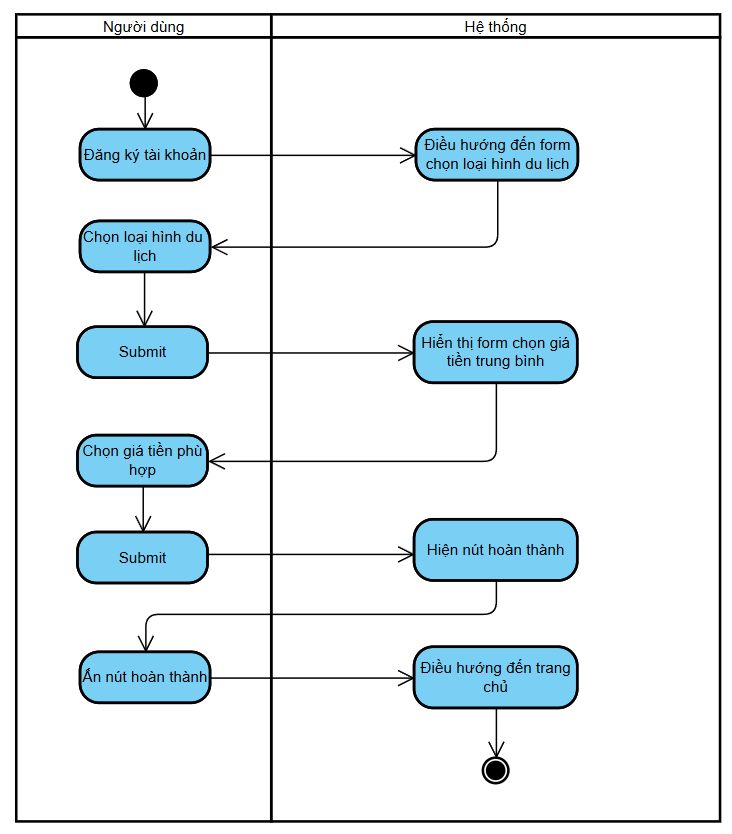
\includegraphics[width=0.5\linewidth]{figures/c3/3-3-3-ad.png}
        &
        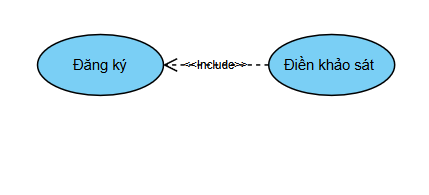
\includegraphics[width=0.45\linewidth]{figures/c3/3-3-3-rd.png} \\
        \hline
    \end{tabular}
\end{table}


\begin{figure}[H]
    \centering
    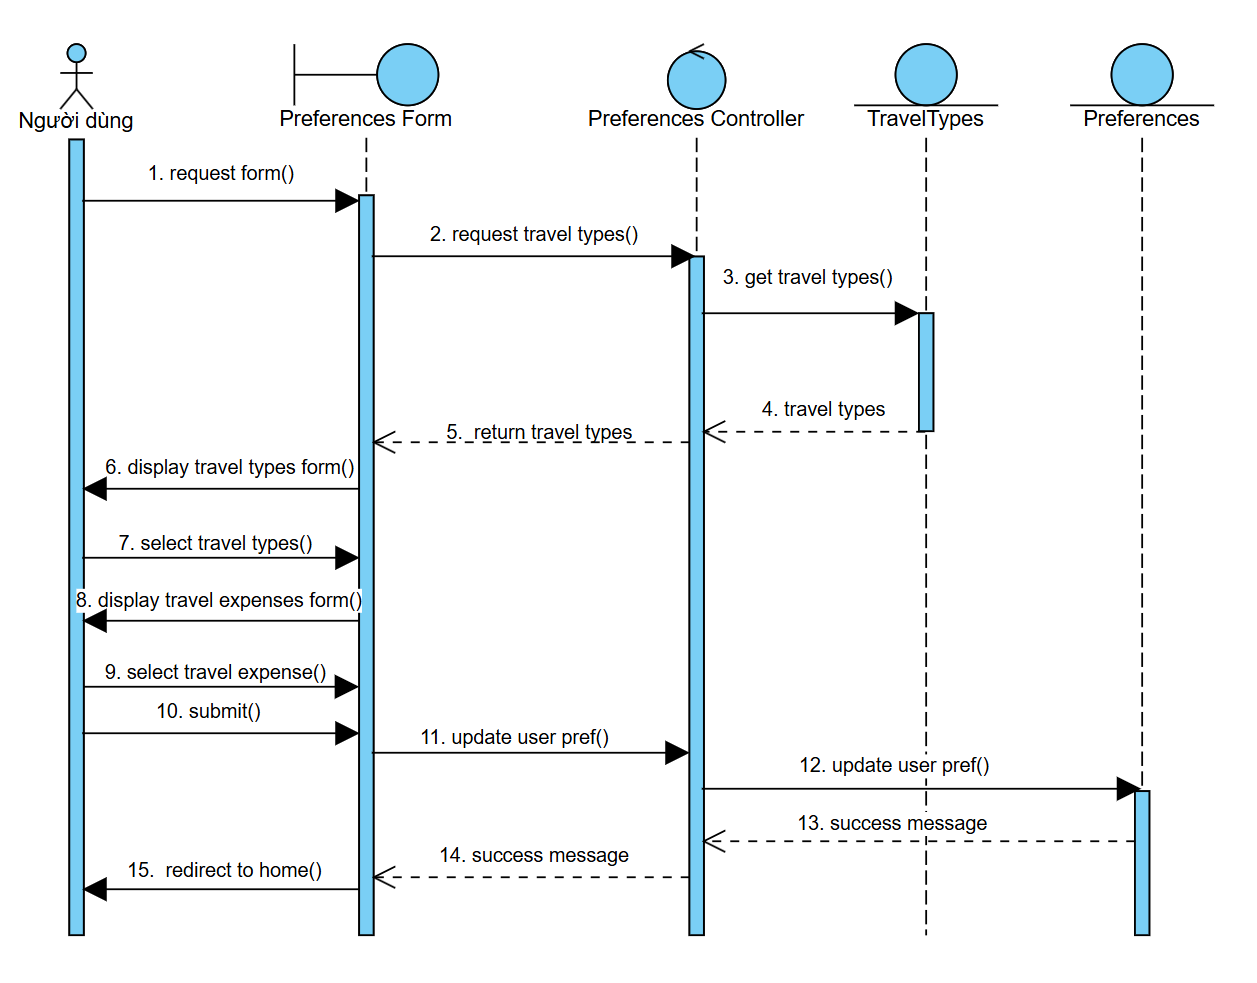
\includegraphics[width=0.85\textwidth]{figures/c3/3-3-3-sd.png}
    \caption{Biểu đồ tuần tự ca sử dụng điền khảo sát sở thích.}
    \label{fig:3-3-3-sequence-diagram}
\end{figure}